\documentclass{article}

\usepackage{graphicx}
\usepackage{hyperref}
\usepackage{apacite}

\title{MAS ISW Assignment 3}
\date{23.11.2020}
\author{Simon Deussen}

\begin{document}
  \pagenumbering{gobble}
  \maketitle
  \pagenumbering{arabic}

  \section*{Task 1: Extract keywords from literature search}

  \begin{itemize}
    \item Swarm robotics \cite{INNOCENTE201980} \cite{OSABA2020101049} \cite{WANG2020} \cite{KONUR2012199} \cite{Winfield_2008}
    \item Self-organization \cite{INNOCENTE201980}
    \item Particle swarm \cite{INNOCENTE201980}
    \item Fire spread modelling \cite{INNOCENTE201980}
    \item Autonomous unmanned aerial vehicles \cite{INNOCENTE201980} \cite{8424838}
    \item Collective behaviour \cite{KHAN2020100715}
    \item Artificial swarming \cite{KHAN2020100715}
    \item Evolutionary framework \cite{KHAN2020100715}
    \item Boids model \cite{KHAN2020100715}
    \item Computational value systems \cite{KHAN2020100715}
    \item Robotics \cite{OSABA2020101049}
    \item Swarm Intelligence \cite{OSABA2020101049}
    \item Bio-inspired computation \cite{OSABA2020101049}
    \item Distributed Computing \cite{OSABA2020101049}
    \item Metaheuristics \cite{OSABA2020101049}
    \item Optimal mass transport (OMT) theory \cite{WANG2020}
    \item Dynamic task allocation \cite{WANG2020} \cite{8424838}
    \item Task allocation \cite{WANG2020} \cite{8424838}
    \item Balanced allocation \cite{WANG2020}
    \item Modelling \cite{Winfield_2008}
    \item Wireless ad hoc network \cite{Winfield_2008}
    \item Controllability \cite{8424838}
    \item Cooperative systems \cite{8424838}
    \item Distributed sensors \cite{8424838}
    \item Mobile robots \cite{8424838}
    \item Multi-robot systems \cite{8424838}
    \item Stability \cite{8424838}
    \item Trajectory control \cite{8424838}
    \item Human operator \cite{8424838}
    \item Ground-based vehicles \cite{8424838}
    \item Three-dimensional space \cite{8424838}
    \item Individual vehicles dynamics \cite{8424838}
    \item Cooperative flight \cite{8424838}
    \item Trajectory generation \cite{8424838}
    \item Adversarial control \cite{8424838}
    \item Distributed monitoring \cite{8424838}
    \item Distributed mapping \cite{8424838}
    \item Theoretical tools \cite{8424838}
    \item Aerial swarm robotics \cite{8424838}
    \item Robot kinematics \cite{8424838}
    \item Robot sensing systems \cite{8424838}
    \item Vehicle dynamics \cite{8424838}
    \item Mathematical model \cite{8424838}
    \item Planning \cite{8424838}
    \item Distributed robot systems \cite{8424838}
    \item Comprehensive learning (CL)
    \item Exploration \cite{LYNN201511}
    \item Exploitation \cite{LYNN201511}
    \item Particle swarm optimization (PSO) \cite{LYNN201511}
    \item Heterogeneous \cite{LYNN201511}
    \item Swarm algorithms \cite{KONUR2012199}
    \item Formal verification \cite{KONUR2012199}
    \item Probabilistic model-checking \cite{KONUR2012199}
  \end{itemize}

\section*{Task 4: Create a mindmap of your taxonomy.}

\begin{figure}[h!]
  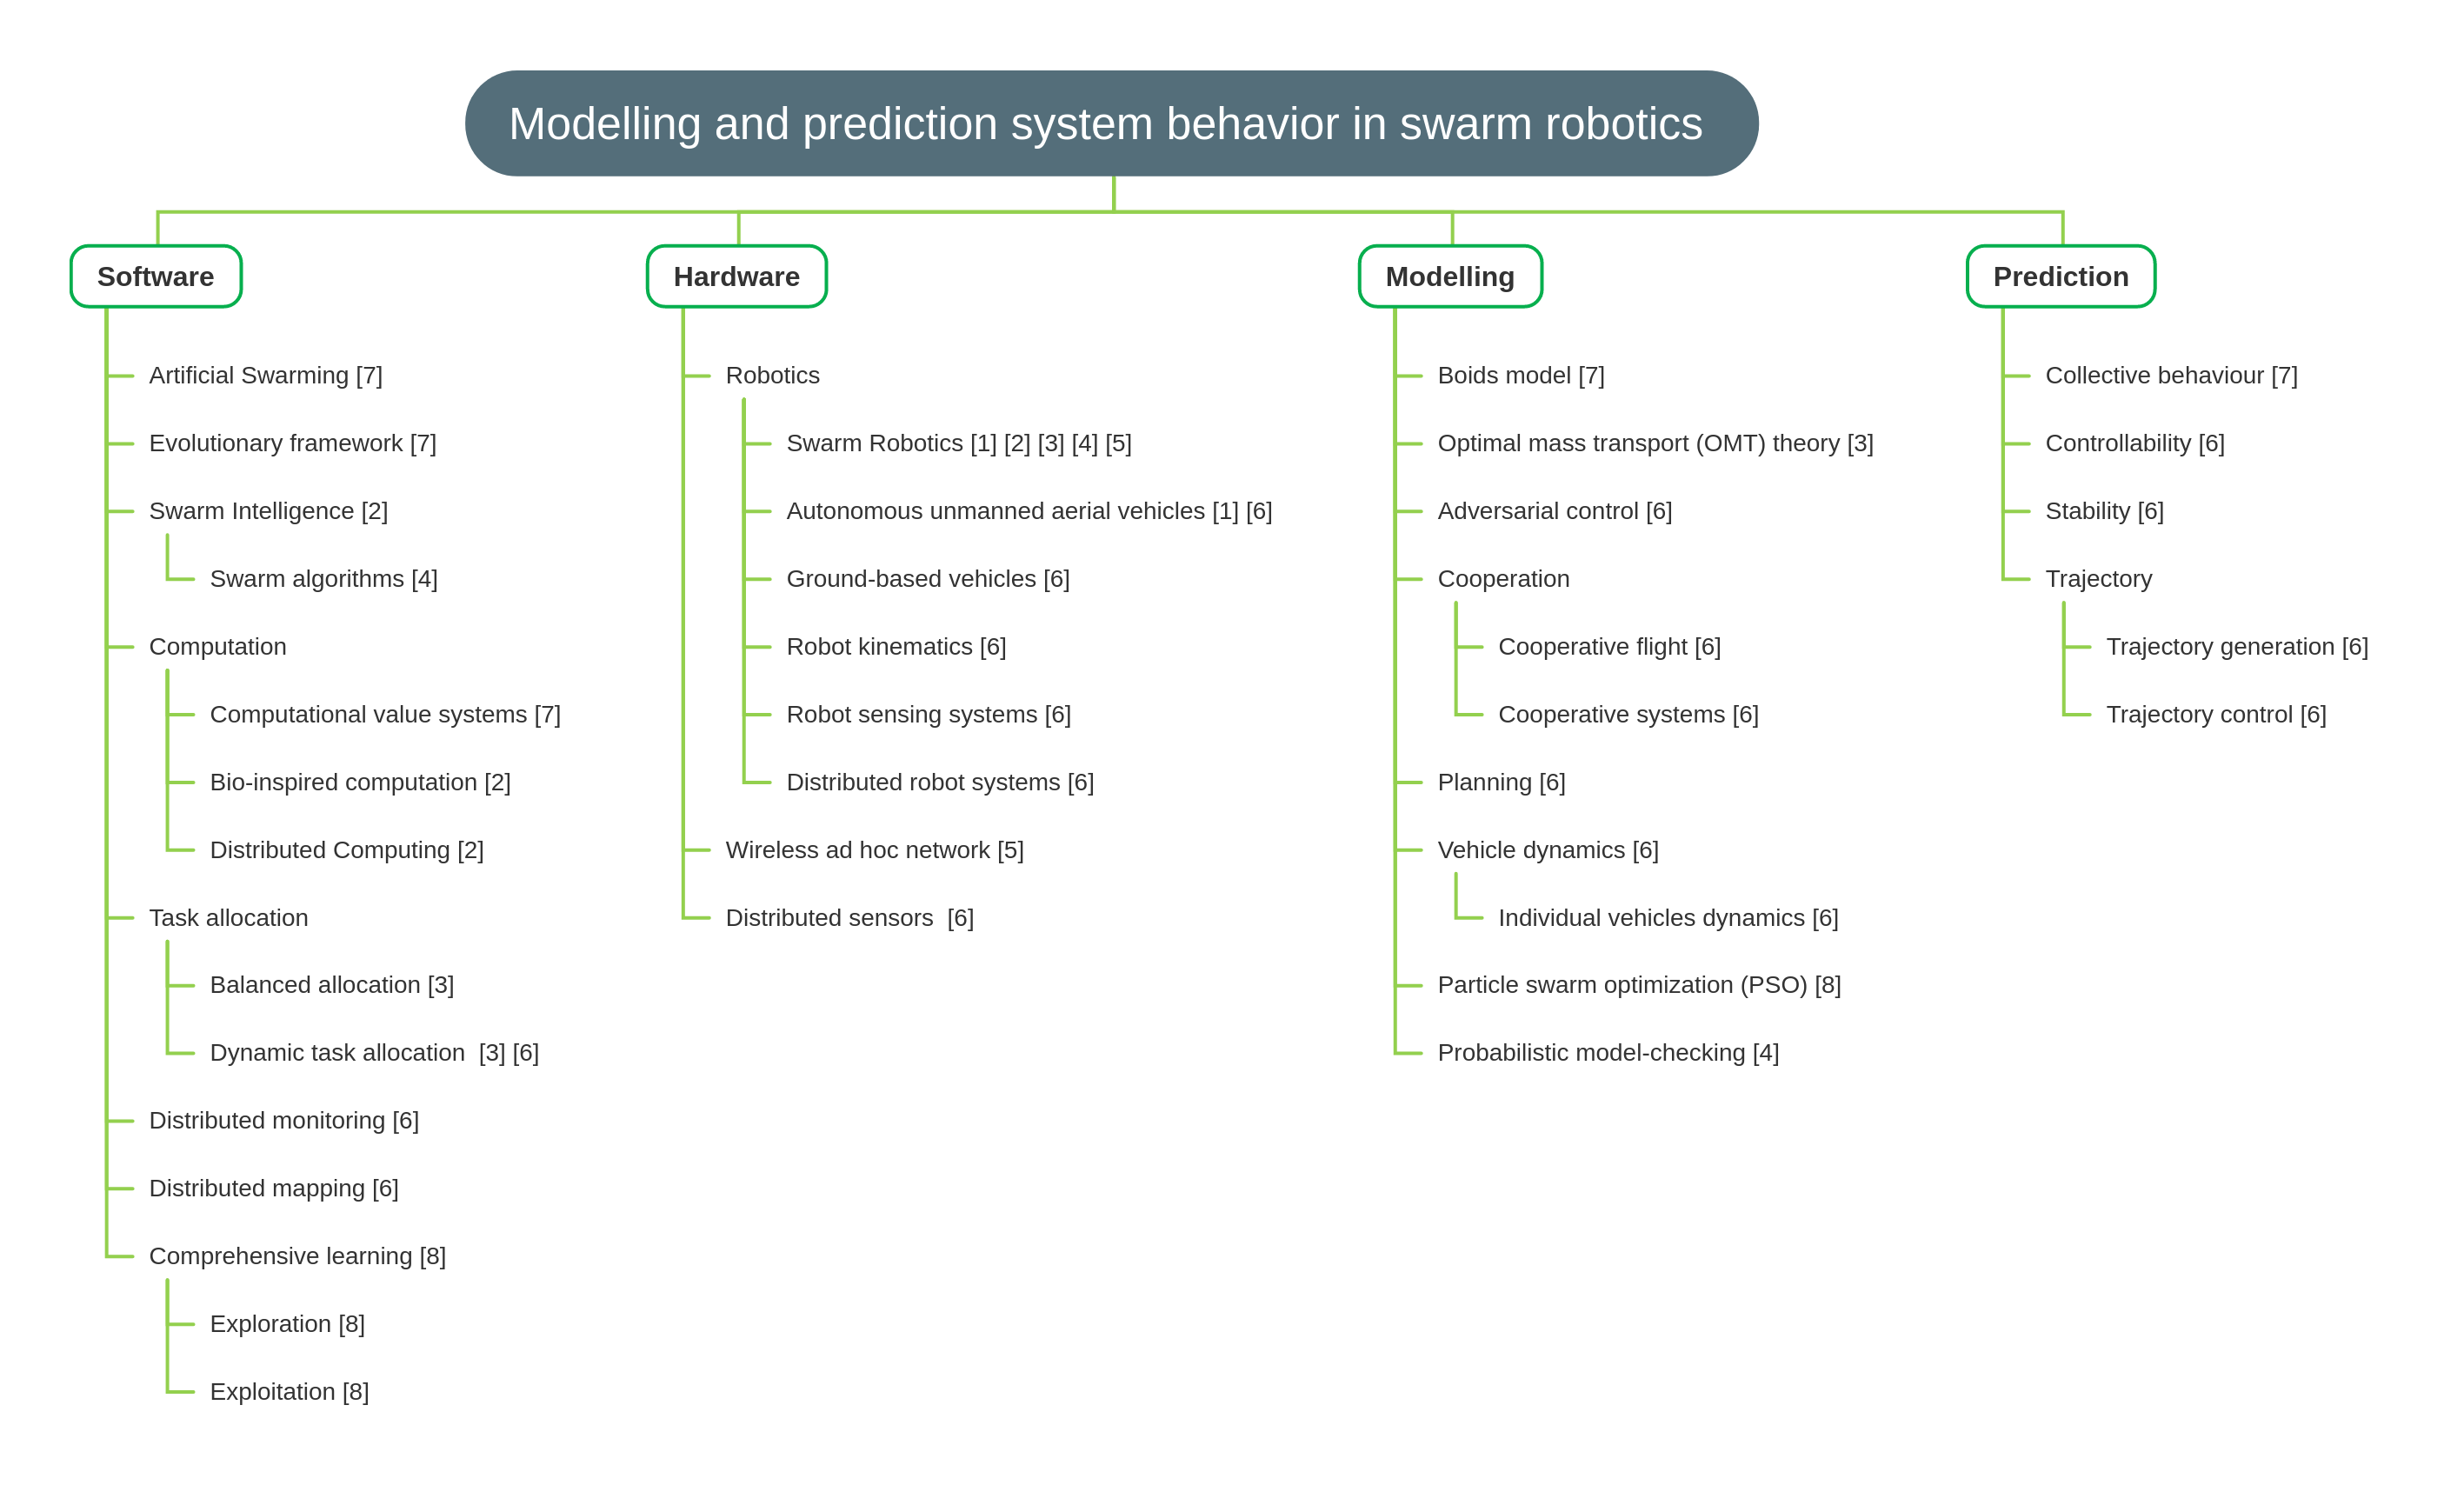
\includegraphics[width=\linewidth]{Robotics.png}
  \caption{Mindmap of the keywords.}
  \label{fig:rob}
\end{figure}

\bibliography{stuff}
\bibliographystyle{apacite}

\end{document}